% DIPOLOMARBEITS TABELLEN DEUTSCH ########################
\newpage
\begin{center}
\textbf{\LARGE DIPLOMA THESIS}

\textbf{Documentation}
\end{center}

%Schülernamen mit Klasse oder Schuljahr
\begin{tikzpicture}
\node[da_dokubox] {
    \textcolor{darkgray}{Authors} \\ 
    \begin{itemize} [itemsep=0pt, topsep=0pt]
        \item[] Jacob Toifl, 5AHIT
        \item[] Michael Schaider, 5AHIT
    \end{itemize}
    \textcolor{darkgray}{Department} \\ 
    \begin{itemize} [itemsep=0pt, topsep=0pt]
        \item[] Information Technology
        \item[] Specialization: 
    \end{itemize}
    \textcolor{darkgray}{Academic year} \\ 
    \begin{itemize} [itemsep=0pt, topsep=0pt]
        \item[] 2025/2026
    \end{itemize}
        \textcolor{darkgray}{Thesis Topic} \\ 
    \begin{itemize} [itemsep=0pt, topsep=0pt]
        \item[] DropIT - structured digital document storage
    \end{itemize}
    \textcolor{darkgray}{Cooperation Partner} \\ 
    \begin{itemize} [itemsep=0pt, topsep=0pt]
        \item[] MBIT Solutions GmbH
    \end{itemize}
}; %node (Rahmen)
\end{tikzpicture}

\vspace{0.5cm}

\begin{tikzpicture}
\node[da_dokubox] {
    \textcolor{darkgray}{Task Description} \\ 
Many companies lack a unified and structured digital document storage system. Contracts and documents are stored unsystematically, resulting in unclear access rights and important information being difficult to find. This leads to missed deadlines, increased search efforts, errors, and security risks.
The goal of this diploma thesis is the development of DropIT – a centralized, user-friendly document storage system with AI-powered classification. The system should automatically recognize and categorize documents, enable fast searching, and protect against missed deadlines through a reminder system. Integration is achieved through Microsoft SharePoint and Entra ID.
    }; %node (Rahmen)
\end{tikzpicture}

\vspace{0.5cm}

\begin{tikzpicture}
\node[da_dokubox] {
    \textcolor{darkgray}{Implementation} \\ 
The system was developed as a modern web application where users can log in with their existing Microsoft company account. Documents are automatically stored in the company's existing SharePoint environment, eliminating the need for separate data storage.
A key feature is the intelligent document recognition: when uploading, the system automatically analyzes the content and identifies the document type – such as a contract, invoice, or proposal. Relevant information like expiration dates or customer names is extracted automatically.
The application is designed to scale easily with growing requirements and can be flexibly extended.
    }; %node (Rahmen)
\end{tikzpicture}

\vspace{0.5cm}

\begin{tikzpicture}
\node[da_dokubox] {
    \textcolor{darkgray}{Results} \\ 
As part of this diploma thesis, a fully functional document management system was developed. Users can log in with their existing Microsoft account and automatically receive the appropriate permissions.
The core of the application is the AI-powered document recognition, which automatically classifies uploaded files and extracts relevant metadata such as expiration dates or contract partners. Documents can be uploaded via drag \& drop into freely definable upload zones, with storage directly in SharePoint.
The implemented full-text search enables quick retrieval of documents by keywords, document type, or date. Additionally, documents can be previewed directly in the application and downloaded.
The integrated reminder system notifies users in advance about expiring deadlines and upcoming tasks, preventing missed deadlines.
\begin{center}
 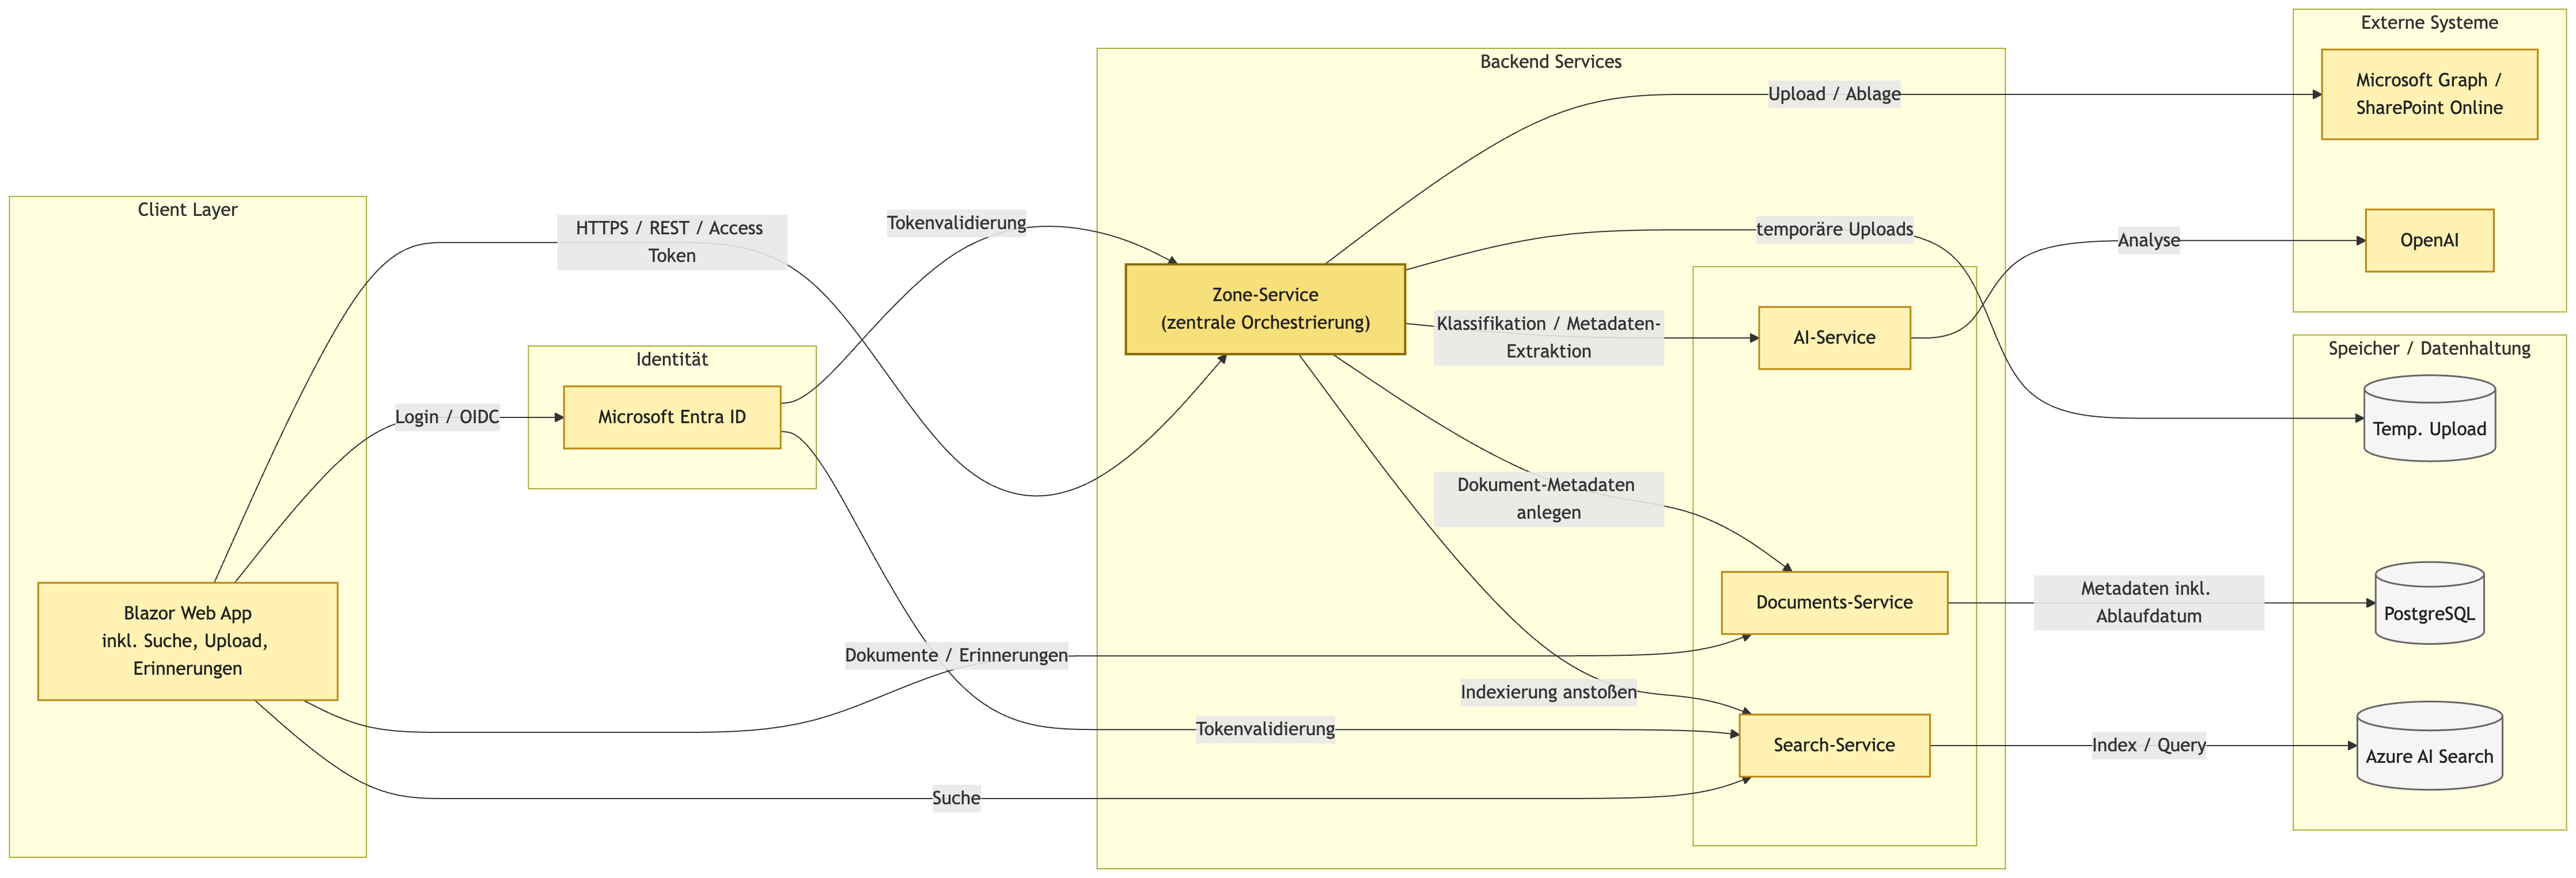
\includegraphics[width=0.95\textwidth]{content/img/4_deployment/systemarchitektur.png}
\end{center}

}; %node (Rahmen)
\end{tikzpicture}